
\noindent \textbf{1. (CRLS 22.2-1)} Simule o funcionamento da BFS no grafo da Figura 22.2(a) do CLRS (segunda edição) a partir do vértice 3, determinando os valores de $d$ e $\pi$ para cada vértice.

\textbf{Resposta:} Inicilizamos os atributos $color$, $d$ e $\pi$ de cada vértice $v \in V$ do grafo com $WHITE$, $\infty$ e $NIL$, respectivamente, conforme a primeira iteração do algoritmo \proc{BFS}, exceto para o nó 3 que é o parâmetro $s$ neste caso, cujo $d = 0$ e sua cor é $GRAY$, conforme pode ser visto em \textbf{a)}.

Colocamos $s$ na fila e, então, visitamos a lista de adjacências de cada vértice a partir de $s$, sendo que $u$ é o vértice retirado da pilha - aquele cuja cor é $BLACK$ ao final do $for$ da linha 12.

Note que o valor de $d$ está dentro de cada vértice do grafo e, a cada novo vértice que descobrimos a partir de $u$, ou seja, aquele que ainda tem a cor $WHITE$, marcamos em seu atributo $\pi$ o seu antecessessor - o próprio $u$ - que destacamos em laranja.

Note, também, que há casos em que nenhum novo vértice é descoberto, como em \textbf{d)}, por exemplo.

Quando a pilha estiver vazia, concluímos a execução do algoritmo. Note que, neste caso, o vértice 1 não pode ser atingido a partir de 3 e, portanto, seu antecessor $\pi$ fica marcado como $NIL$. O vértice $s$ também tem seu antecessor $NIL$, já que é a entrada da busca no grafo e isso ocorre sempre.

As arestas que estão destacadas formam a \textit{breadth-first tree} e o antecessor de cada nó da árvore é dado pelo atributo $\pi$ de cada vértice.

\begin{center}
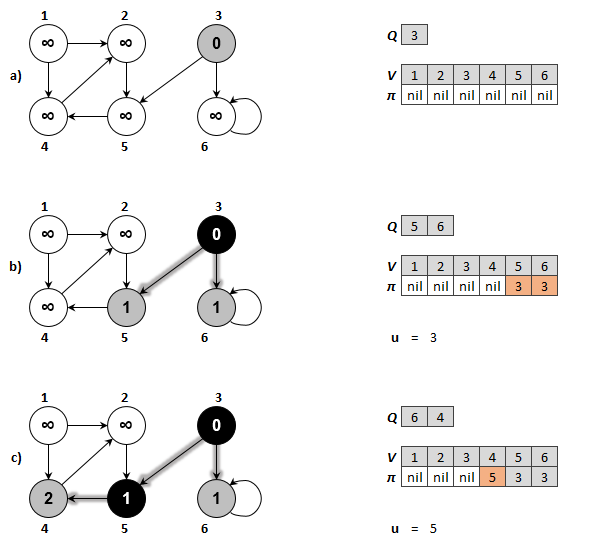
\includegraphics[width=0.8\textwidth]{q7-01-p1.png}
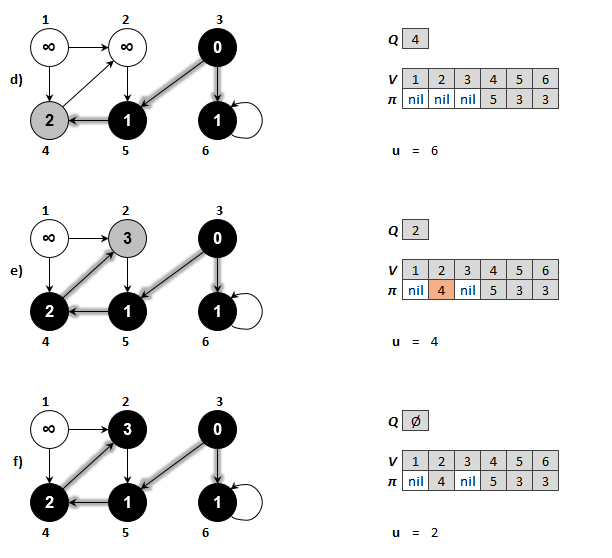
\includegraphics[width=0.8\textwidth]{q7-01-p2.png}
\captionof{figure}{Sequência das operações do algoritmo \proc{BFS}, sendo $s = 3$.}
\label{fig:7.1-1}
\end{center}